
\section{Розділ перший}
Цей документ своренно для тестування latex-стилю для оформлення курсових робіт
за вимогами ВНТУ.

На данний момент стиль підтримує тільки курсові роботи (ДСТУ~3008-95). В
майбутньому (наступному триместрі) планується підтримка курсових проектів
(ГОСТ~2.105-95), і написання документації.
\subsection{Підрозділ перший}
Список того, що необхідно зробити, чи закінчити:
\begin{enumerate}
	\item підтримка бібліографії;
	\item підтримка ненумерованих розділів (аннотація, вступ, і т.п.);
	\item підтримка додатків;
	\item шаблони обов'язкових сторінок (титульний лист, обов'язкові додатки).
\end{enumerate}

\subsubsection{Підпідрозділ перший}

Складний список згідно госту:
\begin{enumerate}
	\item перший рядок першого рівня містить достатьно довгий текст, що повинен
		  перенестися на нову стрічку;
	\item другий рядок першого рівня містить:
	\begin{enumerate}
		\item перший підрядок другого рядка;
		\item другий підрядок другого рядка також містить достатьно довгий
			  текст, що повинен перенестися на нову стрічку;
		\item третій підрядок другого рядка:
	\end{enumerate}
	\item третій рядок третього рівня;
	\item 4;
	\item 5;
	\item 6;
	\item 7;
	\item 8;
	\item 9;
	\item 10;
	\item 11;
	\item 12;
	\item 13;
	\item 14;
	\item 15;
	\item 16;
	\item 17;
	\item 18;
	\item 19;
	\item 20;
	\item 21;
	\item 22;
	\item 23;
	\item 24;
	\item 25;
	\item 26;
	\item 27;
	\item 28;
	\item 29;
	\item 30;
 	\item 31.
% 	\item 32;
% 	\item 33;
% 	\item 34;
% 	\item 35;
% 	\item 36;
% 	\item 37;
%	\item 38;
%	\item 39;
%	\item 40.
\end{enumerate}

Текст після списку. Текст після списку. Текст після списку. Текст після списку. Текст після списку. Текст після списку. Текст після списку.

\begin{figure}[h]
  \centering
  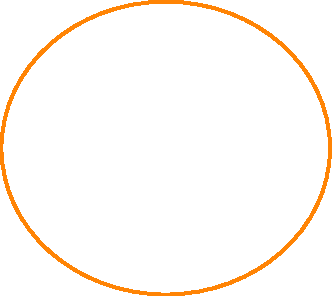
\includegraphics{example}
  \caption{\label{img:img_example}Пример рисунка.}
\end{figure}

Метод Голда\cite{fstbook} получен из метода ван Циттерта\cite{2book}, но
с предположением, что действует он только для положительных чисел.
Восстанавливает по следующему алгоритму\cite{4book,5book,6book}.

Порядок методу дорівнює $p$, якщо існує таке позитивне число $c$, що
\begin{equation}\label{eq:delta}
  \Delta \le ch^{p+1},
\end{equation}

де ${\Delta}$~--- локальна похибка на кроці;

${h}$~--- крок дискретизації;

${p}$~--- порядок методу.

Текст після формули. Текст після формули. Текст після формули. Текст після формули. Текст після формули.